\part{Optimeringsproblemer og Optimalitet}
\label{part:introduction}

\chapter{Matematisk bakgrunn}
\label{chap:mathematical_background}

\section{Grunnleggende lineær algebra}
\subsection{Vektor operasjoner}

\subsubsection{Indre produkt}
Det indre produktet, også kjent som skalarprodukt, er en operasjon som tar to vektorer og gir et tall. 
Dette tallet representerer på mange måter hvordan vektorene "overlapper" med hverandre, og er spesielt nyttig for å måle avstander og vinkler mellom vektorer.

\begin{definition}{Indre produkt}{inner_product}
	Gitt to vektorer \( \symbf{u}, \symbf{v} \in \R^n \), er det indre produktet definert som:

	\[
		\symbf{u} \cdot \symbf{v} = \symbf{u}^\top \symbf{v} = \sum_{i=1}^{n} u_i v_i
	\]

\end{definition}

\begin{remark}{Projeksjon}{projection}
	Projeksjonen av vektoren \( \symbf{u} \) på vektoren \( \symbf{v} \) er gitt ved:
	\[
		\operatorname{proj}_{\symbf{v}}(\symbf{u}) = \frac{\symbf{u} \cdot \symbf{v}}{\norm{\symbf{v}}^2} \symbf{v}
	\]
	Dette gir oss en ny vektor som er parallell med \( \symbf{v} \) og representerer den delen av \( \symbf{u} \) som "går i retning" av \( \symbf{v} \).
\end{remark}

\subsubsection{Ytre produkt (tensorprodukt)}
Ytre produktet er en operasjon som tar to vektorer og lager en matrise.
\begin{definition}{Ytre produkt}{outer_product}
	Gitt to vektorer \( \symbf{u} \in \R^m \) og \( \symbf{v} \in \R^n \), er det ytre produktet definert som:
	\[
		\symbf{u} \otimes \symbf{v} = \symbf{u} \; \symbf{v}^\top =
		\begin{bmatrix}
			u_1v_1 & u_1v_2 & \cdots & u_1v_n \\
			u_2v_1 & u_2v_2 & \cdots & u_2v_n \\
			\vdots & \vdots & \ddots & \vdots \\
			u_mv_1 & u_mv_2 & \cdots & u_mv_n
		\end{bmatrix}
	\]
\end{definition}

\subsubsection{Norm}
Norm er et mål på størrelsen eller lengden av en vektor. Den mest brukte normen er den euklidiske normen, som er definert under.

\begin{definition}{Norm}{norm}
	Gitt en vektor \( \symbf{x} \in \R^n \), er normen definert som:
	\[
		\norm{\symbf{x}} = \sqrt{\symbf{x}^\top \symbf{x}} = \sqrt{\sum_{i=1}^{n} x_i^2}
	\]
\end{definition}

Andre viktige normer inkluderer:
\begin{align*}
	\tag{Euklidisk norm} \norm{\symbf{x}}_2 &= \sqrt{\sum_{i=1}^{n} x_i^2} \\
	\tag{Manhattan norm} \norm{\symbf{x}}_1 &= \sum_{i=1}^{n} |x_i| \\
	\tag{Max norm} \norm{\symbf{x}}_\infty &= \max_{i=1,\ldots,n} |x_i|
\end{align*}


\section{Mengder}
\subsection{Baller}
En åpen ball i \(\R^d\) er en mengde av punkter \(\mathbf{x}\) som ligger innenfor en viss avstand \(r\) fra et sentrum \(\mathbf{x_0}\).

Den er definert ved hjelp av den euklidiske normen \(\norm{\cdot}\), som måler avstanden mellom to punkter i rommet.

\begin{definition}{Åpen Ball}{open_ball}
	En åpen ball \(B(\mathbf{x}_0, r)\) i \(\R^d\) med sentrum \(\mathbf{x}_0\) og radius \(r\) er definert som:
	\[
		B(\mathbf{x}_0, r) = \{ \mathbf{x} \in \R^d : \norm{\mathbf{x} - \mathbf{x}_0} < r\}
	\]
	\begin{itemize}
		\item \(B(\mathbf{x}_0, r)\) er åpen hvis den ikke inkluderer grensen.
		\item \(B(\mathbf{x}_0, r)\) er lukket hvis den inkluderer grensen.
	\end{itemize}
\end{definition}

\subsection{Nivåsett}
Intuitivt er nivåsettet til en funksjon \( f \) i et punkt \( y \) mengden av alle punkter \( x \) som har samme eller lavere verdi enn \( y \) under \( f \).
\begin{definition}{Nivåsett}{level_set}
	\(f: \Omega \to \overline{\R}\) er en funksjon. Vi definerer nivåsettet til \(f\) i punktet \(y \in \R\) som:
	\[
		\mathcal{L}_f(y) = \{x \in \Omega | f(x) = y\}.
	\]
\end{definition}

\subsection{Åpen mengde}

\begin{definition}{Åpen mengde}{open_set}
	En mengde \(A \subset \R^n\) er åpen hvis for alle \(x \in A\) finnes det en \(\varepsilon > 0\) slik at \(B(x, \varepsilon) \subset A\).
	\[
		\forall x \in A, \exists \varepsilon > 0 \text{ s.a. } B(x, \varepsilon) \subset A
	\]
\end{definition}

\subsection{Lukket mengde}
En lukket mengde er en mengde som inneholder alle sine grensepunkter \enquote{$[$}, \enquote{$]$}.
\begin{definition}{Lukket mengde}{closed_set}
	En mengde \(A \subset \R^n\) er lukket hvis komplementet \(A^c\) er åpent.
	\[
		A \text{ er lukket} \Leftrightarrow A^c \text{ er åpen}
	\]
\end{definition}

\subsection{Begrenset mengde}

En mengde er begrenset hvis den ikke strekker seg til uendelig langt i noen retning.
Intuitivt kan vi si at en mengde er begrenset hvis den kan plasseres innenfor en kule med endelig radius.

\begin{definition}{Begrenset mengde}{bounded_set}
	En mengde \(A \subset \R^n\) er begrenset hvis det finnes en \(R > 0\) slik at
	\[
		\norm{x} \leq R \quad \forall x \in A
	\]
\end{definition}

\subsection{Kompakt mengde}

En kompakt mengde er en mengde som er både lukket og begrenset. Dette betyr at den er avgrenset og inneholder alle sine grenseverdier.

\begin{definition}{Kompakt mengde}{compact_set}
	En mengde \(A \subset \R^n\) er kompakt hvis den er lukket og begrenset.
	\[
		A \text{ er kompakt} \Leftrightarrow A \text{ er lukket og begrenset}
	\]
\end{definition}

\section{Funksjoner}
\subsection{Nedre semi-kontinuerlige funksjoner}
En nedre semikontinuerlig funksjon (\textit{lower semi-continuous function}) er en funksjon som ikke har plutselige "hopp nedover".

Tenk deg at du nærmer deg et punkt \( \symbf{x_0} \) fra alle mulige retninger:
\begin{itemize}
	\item Verdien av funksjonen i \( \symbf{x_0} \) vil ikke være høyere enn verdiene du ser når du kommer nærmere.
	\item Funksjonen kan ha "hopp oppover".
\end{itemize}


\begin{definition}{Nedre semi-kontinuerlig funksjoner}{lsc}
	\(f: \Omega (\subset \R^d) \to \overline{\R}\) være en funksjon. Vi sier at \(f\) er nedre semi-kontinuerlig (lsc) i punktet \(x_0\) hvis for alle \(\varepsilon > 0\) finnes det en \(\delta > 0\) slik at
	\[
		f(x) > f(x_0) - \varepsilon \quad \text{for alle} \quad x \in B(x_0, \delta).
	\]
	\begin{enumerate}
		\item \(f\) er (lsc) i \(x_0\) hvis det for alle \(\alpha \in \R\) er mengden \(\mathcal{L}_f(\alpha) = \{x | f(x) < \alpha \} \text{ er åpen i } \R^d\)
		\item \(f\) er (lsc) i \(x_0 \in X\) hvis og bare hvis: \(\liminf_{x \to x_0} f(x) \geq f(x_0)\).
	\end{enumerate}
\end{definition}
\begin{example}{Eksempel på en nedre semi-kontinuerlig funksjon}{lsc}
	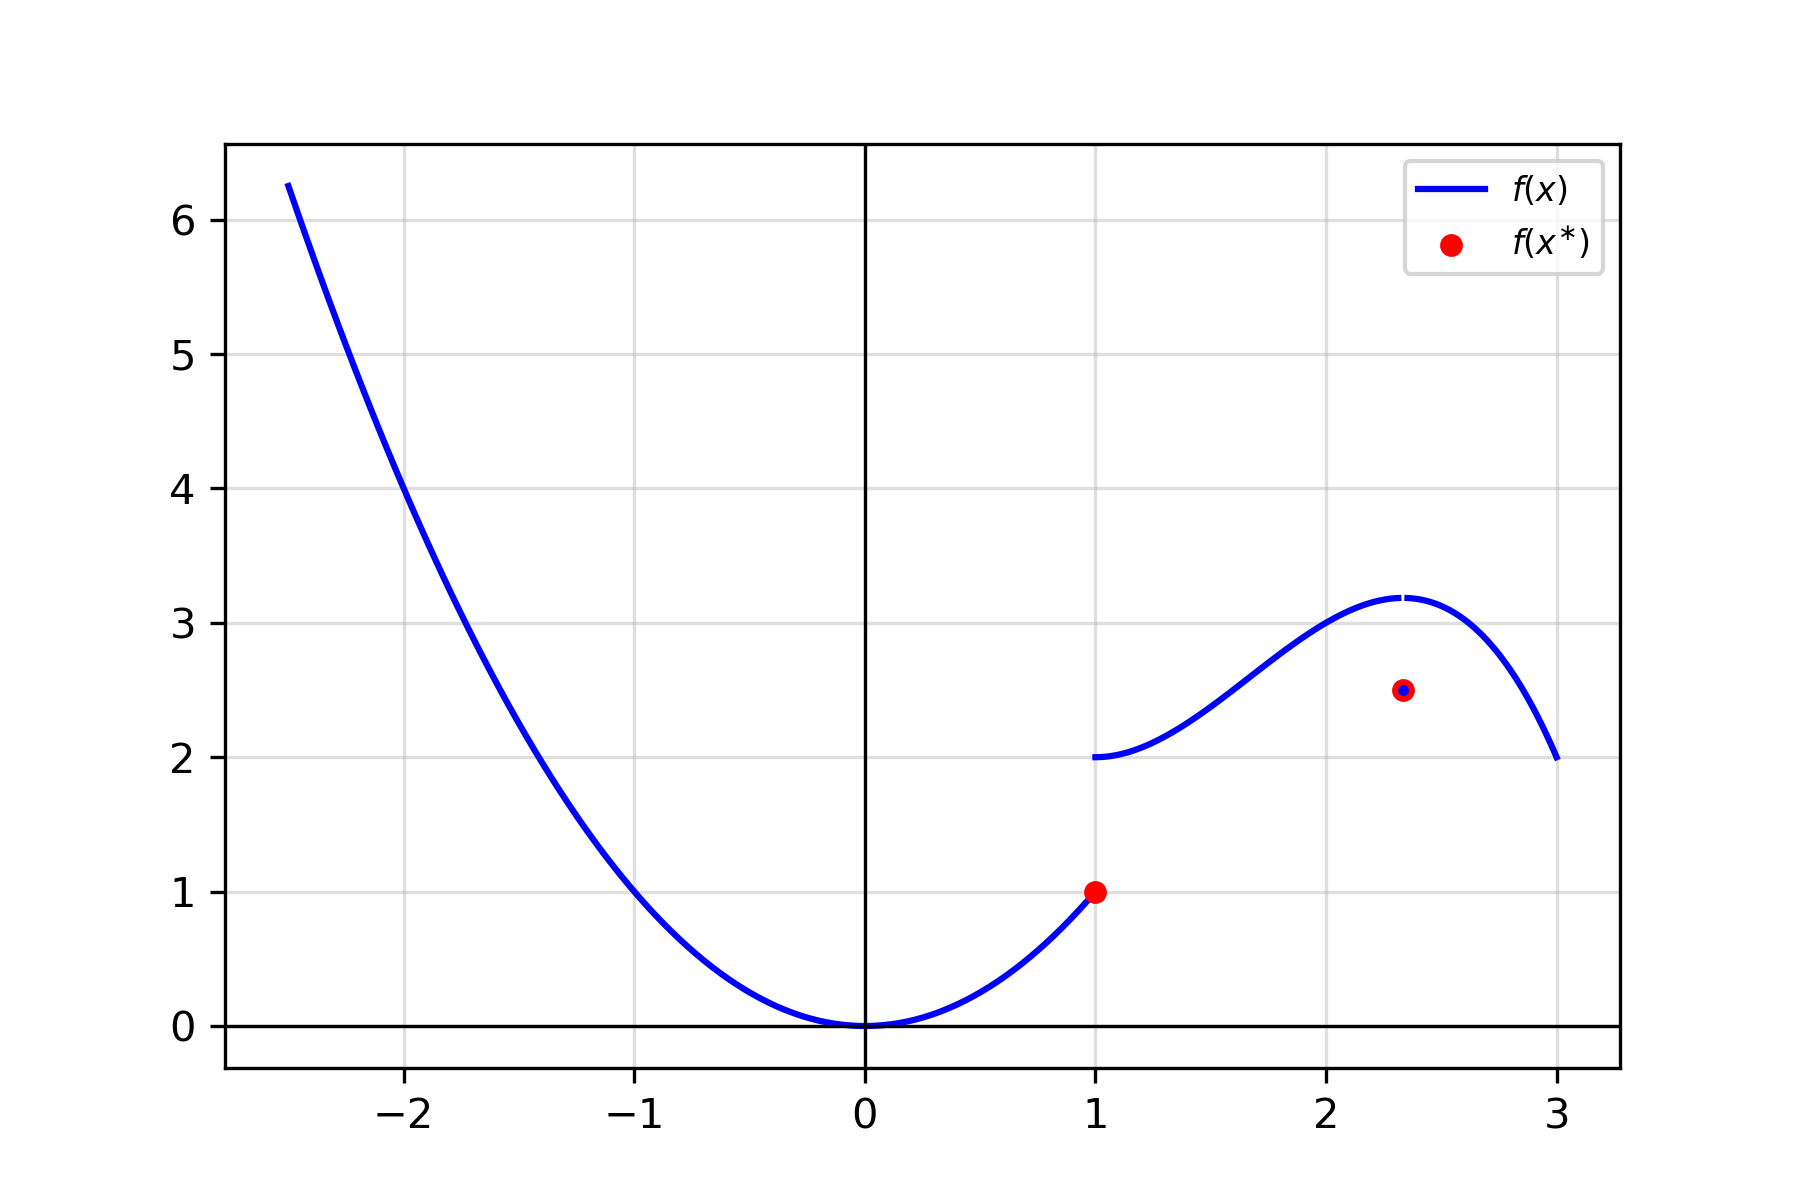
\includegraphics[width=0.5\textwidth]{figures/example_lsc.png}
\end{example}

\subsection{Koersivitet}
En koersiv funksjon er intuitivt en funksjon som "går mot uendelig" når vi beveger oss mot kanten av definisjonsmengden hvor \( f \) er definert.

\begin{definition}{Koersivitet}{coercive}
	En funksjon \(f: \Omega \to \R\) er koersiv hvis for alle \(y \in \R\) er nivåmengden \(\mathcal{L}_f(y) = \{x \in \Omega | f(x) \leq y\}\) kompakt.

	\[
		\lim_{\norm{x} \to +\infty} f(x) = +\infty
	\]
\end{definition}

\subsection{Konveksitet, kvasi-konveksitet og konvekse mengder}

Konveksitet er et viktig begrep i optimering og matematikk generelt. Det refererer til formen på en funksjon eller en mengde.
\begin{itemize}
	\item En konveks funksjon har en bue som vender oppover.
	\item En konkav funksjon har en bue som vender nedover.
	\item En konveks mengde er en mengde der enhver linje mellom to punkter i mengden også ligger helt innenfor mengden.
\end{itemize}

\begin{definition}{Konveks funksjon}{convex_function}
	En funksjon \(f: \R^n \to \R\) er:
	\begin{align*}
		f(\lambda x + (1-\lambda)y) & \leq \lambda f(x) + (1-\lambda)f(y) \quad \forall x, y \in \R^n, \lambda \in [0, 1] \tag{Konveks}                  \\
		f(\lambda x + (1-\lambda)y) & < \lambda f(x) + (1 - \lambda)f(y) \quad \forall x, y \in \R^n, \lambda \in (0, 1), x \neq y \tag{Strengt konveks}
	\end{align*}
\end{definition}

\begin{remark}{Konveksitet med indre-produkt notasjon}{convex_inner_product}
	En funksjon  \(f: \R^n \to \R\) er konveks hvis og bare hvis:
	\[
		f(y) - f(x) \geq  \langle \nabla f(x), y - x \rangle
	\]
	for alle  \(x, y \in \R^n\).
\end{remark}


\begin{remark}{Kvasi-konveks}{quasi_convex}
	En funksjon \(f: \R^d \to \R\) er kvasi-konveks hvis for alle \(x, y \in \R^n\) og \(\lambda \in (0, 1)\) har vi:

	\[
		f(\lambda x + (1 - \lambda)y) \leq \max\{f(x), f(y)\}
	\]

	En alternativ definisjon er at en funksjon er kvasi-konveks hvis alle nivåsettene er konvekse.

	\[
		\mathcal{L}_f(y) = \{x \in \R^n | f(x) \leq y\} \quad \text{er konveks for alle} \quad y \in \R
	\]

	\[
		\boxed{\underbrace{\forall \alpha \in \R, \mathcal{L}_f(\alpha) \text{ er konveks}}_{f \text{ er kvasi-konveks }}\Longleftrightarrow \forall x, y \in \R^d,\lambda \text{ s.a. } f(\lambda x + (1-\lambda)y) \leq \max \{ f(x), f(y) \}}
	\]
\end{remark}

\begin{definition}{Konveks sett}{convex_set}
	En mengde \(C \subset \R^n\) er (strengt) konveks når:

	\begin{align*}
		\lambda x + (1 - \lambda)y & \in C \quad \forall \; x, y \in C, \lambda \in [0, 1] \tag{Konveks}                   \\
		\lambda x + (1 - \lambda)y & \in C \quad \forall \; x, y \in C, \lambda \in (0, 1), x \neq y \tag{Strengt konveks}
	\end{align*}

\end{definition}

\begin{definition}{Konveks kombinasjon}{convex_combination}
	En konveks kombinasjon av punkter $x_1, x_2, \ldots, x_n$ i $\mathbb{R}^d$ er ethvert punkt på formen:
	\[
		\sum_{i=1}^n \lambda_i x_i \quad \text{der} \quad \lambda_i \geq 0, \sum_{i=1}^n \lambda_i = 1
	\]
\end{definition}

\begin{remark}{Karakterisering av deriverbare konvekse funksjoner}{convex-characterization}
	For en deriverbar funksjon  \(f: \R^n \to \R\) er følgende ekvivalente:
	\begin{itemize}
		\item  \(f\) er konveks
		\item For alle  \(x, y \in \R^n\) gjelder:
		      \[
			      f(y) \geq f(x) + \nabla f(x)^\top (y - x)
		      \]
	\end{itemize}
\end{remark}

\section{Ekvivalente utsagn for konvekse funksjoner}

La \(f:\mathbb{R}^n \to \mathbb{R}\) være en funksjon. Følgende utsagn er ekvivalente:
\begin{table}[H]
	\centering
	\small
	\begin{tabularx}{\textwidth}{|X|X|X|}
		\rowcolor{rem-color!25}
		\textbf{Ekvivalente Utsagn} & \textbf{Matematisk Definisjon} & \textbf{Forklaring og Intuisjon} \\
		\hline
		Geometrisk & 
		\( f(\lambda \symbf{x} + (1-\lambda)\symbf{y}) \le \lambda f(\symbf{x}) + (1-\lambda)f(\symbf{y}) \)  
		for alle \( \symbf{x},\symbf{y} \) i domenet og \( \lambda \in [0,1] \)
		& Grafen til \( f \) ligger under eller på sekantlinjene som forbinder to punkter på grafen. \\
		\hline
		Epi-graf &
		\(\operatorname{epi}(f) = \{ (\symbf{x},t)\in\mathbb{R}^n\times\mathbb{R} : f(\symbf{x})\le t \}\) er konveks.
		& Enhver konveks kombinasjon av punkter i epi-grafen tilhører også epi-grafen. \\
		\hline
		Første orden &
		\( f(\symbf{y}) \ge f(\symbf{x}) + \nabla f(\symbf{x})^\top (\symbf{y}-\symbf{x}) \)
		(gjelder dersom \( f \) er deriverbar)
		& Tangentplanet i ethvert punkt underestimerer \( f \) globalt, for alle \( \symbf{x},\symbf{y} \) i domenet. \\
		\hline
		Global optimalitet &
		Hvis \( f \) er konveks, er hvert lokalt minimum et globalt minimum.
		& En konsekvens av konveksitet: en konveks funksjon kan ikke ha ``isolerte'' lokale minima. (Merk at enkelte ikke-konvekse, quasi-konvekse funksjoner også kan ha denne egenskapen.) \\\hline
		Andre orden &
		\( \nabla^2 f(\symbf{x}) \succeq 0 \) for alle \( \symbf{x} \) i domenet 
		(dersom \( f \) er to ganger deriverbar)
		& Hessianmatrisen er positiv semidefinit, noe som via Taylorutvidelsen tilsier at funksjonen ikke ``bøyer'' seg nedover. \\
		\hline
		Subgradient &
		For alle \( \symbf{x} \) er \( \partial f(\symbf{x}) \neq \varnothing \) og for hvert \( s \in \partial f(\symbf{x}) \) gjelder 
		\( f(\symbf{y}) \ge f(\symbf{x}) + s^\top (\symbf{y}-\symbf{x}) \)
		& Selv om \( f \) ikke er deriverbar, gir tilstedeværelsen av subgradienter en lineær underestimering som karakteriserer konveksitet. 
		\\
		\hline
	\end{tabularx}
	\caption{Ekvivalente karakteriseringer av konvekse funksjoner, ordnet etter kompleksitet.}
	\label{tab:convex_equivalence}
\end{table}

\section{Geometriske objekter}
\subsection{Simplex}
Et simplex er en geometrisk figur som kan forstås som den enkleste formen i et gitt antall dimensjoner. For eksempel er et 0-simplex et punkt, et 1-simplex er en linje, et 2-simplex er en trekant, og så videre.

\begin{definition}{Simplex}{simplex}
	Et simplex i \( \mathbb{R}^n \) er et \( n \)-dimensjonalt objekt laget av \( n+1 \) punkter (hjørner) som ikke ligger i samme hyperplan.

	\begin{figure}[H]
		\centering
		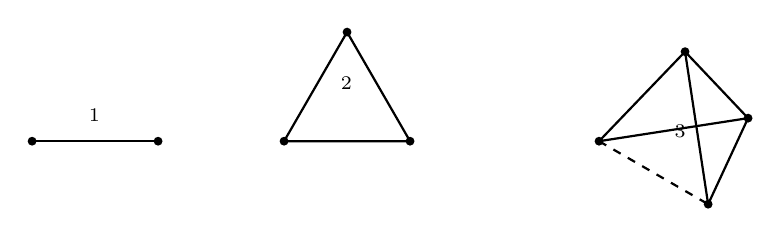
\begin{tikzpicture}[scale=0.8]
			% R1 simplex (line)
			\begin{scope}[shift={(-4,0)}]
				\draw[thick] (0,0) -- (2,0);
				\fill (0,0) circle (2pt);
				\fill (2,0) circle (2pt);
				\node[above] at (1,0) {$\R^1$};
			\end{scope}

			% R2 simplex (triangle)
			\begin{scope}[shift={(0,0)}]
				\draw[thick] (0,0) -- (2,0) -- (1,1.732) -- cycle;
				\fill (0,0) circle (2pt);
				\fill (2,0) circle (2pt);
				\fill (1,1.732) circle (2pt);
				\node[above] at (1,0.5) {$\R^2$};
			\end{scope}

			% R3 simplex (tetrahedron)
			\begin{scope}[shift={(5,0)}, x={(0.866cm,-0.5cm)}, y={(0.866cm,0.5cm)}, z={(0cm,1cm)}]
				% Back triangle
				\draw[thick,dashed] (0,0,0) -- (2,0,0);
				\draw[thick] (2,0,0) -- (1,1.732,0) -- (0,0,0);
				% Vertical edges to top point
				\draw[thick] (0,0,0) -- (1,0.577,1.633);
				\draw[thick] (2,0,0) -- (1,0.577,1.633);
				\draw[thick] (1,1.732,0) -- (1,0.577,1.633);
				% Points
				\fill (0,0,0) circle (2pt);
				\fill (2,0,0) circle (2pt);
				\fill (1,1.732,0) circle (2pt);
				\fill (1,0.577,1.633) circle (2pt);
				\node[above] at (1,0.5,0) {$\R^3$};
			\end{scope}
		\end{tikzpicture}
		\caption{Simplex i ulike dimensjoner.}
	\end{figure}
\end{definition}

\chapter{Konveksitet}

\section{Konvekse Mengder}

\subsection{Definisjon}
\begin{definition}{Konveks Mengde}{convex_set}
    En mengde $C \subset \mathbb{R}^n$ er \textbf{konveks} hvis, for ethvert par punkter $x, y \in C$, ligger hele linjesegmentet som forbinder dem i $C$. Formelt:
    \[
    x, y \in C \quad \Longrightarrow \quad \alpha x + (1-\alpha) y \in C \quad \text{for alle}~\alpha \in [0, 1].
    \]
    Ekvivalent kan man si at enhver konveks kombinasjon av punkter i $C$ forblir i $C$.
\end{definition}

\begin{figure}[htb]
    \centering
    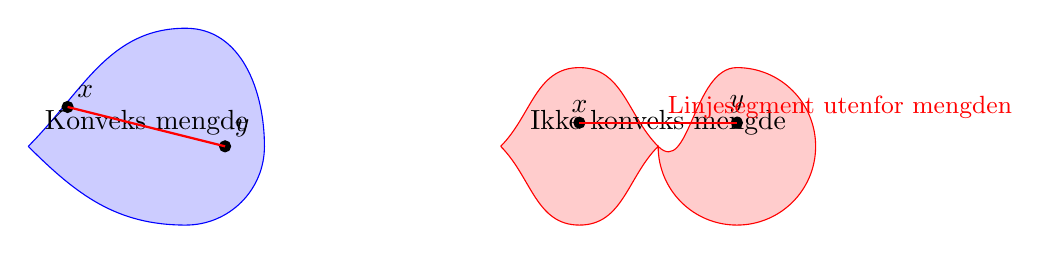
\begin{tikzpicture}
        % Convex set
        \draw[fill=blue!20, draw=blue] (0,0) to[out=45, in=180] (2,1.5) to[out=0, in=90] (3,0) to[out=270, in=0] (2,-1) to[out=180, in=315] (0,0);
        \node at (1.5, 0.3) {Konveks mengde};
        \filldraw[black] (0.5,0.5) circle (2pt) node[above right] {$x$};
        \filldraw[black] (2.5,0) circle (2pt) node[above right] {$y$};
        \draw[thick, red] (0.5,0.5) -- (2.5,0);
        
        % Non-convex set
        \begin{scope}[xshift=6cm]
            \draw[fill=red!20, draw=red] (0,0) to[out=45, in=180] (1,1) to[out=0, in=135] (2,0) to[out=315, in=180] (3,1) to[out=0, in=90] (4,0) to[out=270, in=0] (3,-1) to[out=180, in=270] (2,0) to[out=225, in=0] (1,-1) to[out=180, in=315] (0,0);
            \node at (2, 0.3) {Ikke-konveks mengde};
            \filldraw[black] (1,0.3) circle (2pt) node[above] {$x$};
            \filldraw[black] (3,0.3) circle (2pt) node[above] {$y$};
            \draw[thick, red] (1,0.3) -- (3,0.3);
            \node[red, right] at (2,0.5) {\small Linjesegment utenfor mengden};
        \end{scope}
    \end{tikzpicture}
    \caption{Illustrasjon av konvekse og ikke-konvekse mengder}
    \label{fig:convex_sets}
\end{figure}


\subsection{Eksempler}
\begin{example}{Vanlige Konvekse Mengder}{common_convex_sets}
    \begin{itemize}
        \item \textbf{Euklidske Kuler}: $\bigl\{ x : \|x - x_0\|\le r \bigr\}$ er konvekse fordi linjesegmenter mellom to punkter i en kule forblir inni.
        \item \textbf{Polyedre}: $\{x : A x \le b\}$ (ulikheter forstått komponentvis) er konvekse. Polytoper og simplekser er spesielle eksempler.
        \item \textbf{Affine Underrom}: $\{x : A x = b\}$ er konvekse.
        \item \textbf{Halvrom}: $\{x \in \mathbb{R}^n : a^T x \leq b\}$ er konvekse.
        \item \textbf{Kjegler}: $\{tx : t \geq 0, x \in C\}$ der $C$ er konveks er konvekse.
    \end{itemize}
\end{example}

\subsection{Operasjoner som Bevarer Konveksitet}
\begin{theorem}{Konveksitetsbevarende Operasjoner}{convexity_preserving}
    Følgende operasjoner bevarer konveksitet av mengder:
    \begin{itemize}
        \item \textbf{Snitt}: Snittet av enhver samling konvekse mengder er konveks.
        \item \textbf{Lineære eller Affine Avbildninger}: Hvis $T$ er en lineær (eller affin) transformasjon, og $C$ er konveks, er $T(C)$ konveks.
        \item \textbf{Minkowski Sum}: For konvekse $C_1,C_2$, er Minkowski-summen $\{x_1 + x_2 : x_1\in C_1, x_2\in C_2\}$ konveks.
        \item \textbf{Skalering og Translasjon}: For enhver $\alpha \in \mathbb{R}$ og $b \in \mathbb{R}^n$, er både $\alpha C$ og $C + b$ konvekse.
    \end{itemize}
\end{theorem}

\subsection{Ekstremalpunkter, Flater og Separasjon}
\begin{definition}{Ekstremalpunkt}{extreme_point}
    Et \textbf{ekstremalpunkt} i en konveks mengde $C$ er et punkt som ikke ligger i noe åpent linjesegment inneholdt i $C$ (bortsett fra det trivielle segmentet som starter og slutter i punktet selv).
\end{definition}

\begin{theorem}{Separasjonsteoremet}{separation_theorem}
    La $C$ og $D$ være disjunkte ikke-tomme konvekse mengder i $\mathbb{R}^n$.
    \begin{enumerate}
        \item Hvis $C$ er åpen, eksisterer det en ikke-null $p \in \mathbb{R}^n$ og $\alpha \in \mathbb{R}$ slik at $p^T x < \alpha \leq p^T y$ for alle $x \in C$ og $y \in D$.
        \item Hvis $C$ og $D$ er lukket og minst én er kompakt, eksisterer det en ikke-null $p \in \mathbb{R}^n$ og $\alpha, \beta \in \mathbb{R}$ slik at $p^T x \leq \alpha < \beta \leq p^T y$ for alle $x \in C$ og $y \in D$.
    \end{enumerate}
\end{theorem}

\begin{figure}[htb]
    \centering
    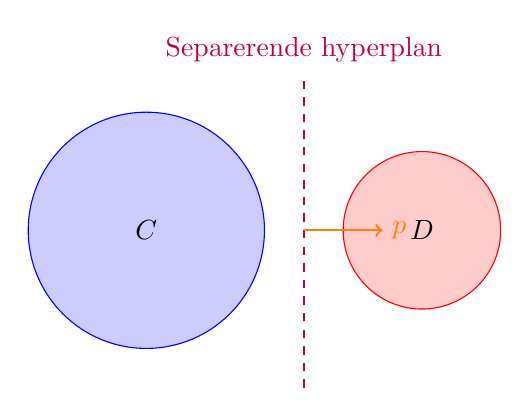
\begin{tikzpicture}
        % Første mengde (konveks)
        \draw[fill=blue!20, draw=blue] (0,0) circle (1.5);
        \node at (0, 0) {$C$};
        
        % Andre mengde (konveks)
        \draw[fill=red!20, draw=red] (3.5,0) circle (1);
        \node at (3.5, 0) {$D$};
        
        % Separerende hyperplan
        \draw[thick, dashed, purple] (2,-2) -- (2,2);
        \node[purple] at (2, 2.3) {Separerende hyperplan};
        
        % Normalvektor til hyperplanet
        \draw[->, thick, orange] (2,0) -- (3,0);
        \node[orange, right] at (3, 0) {$p$};
    \end{tikzpicture}
    \caption{Separasjon av to konvekse mengder med et hyperplan}
    \label{fig:separation}
\end{figure}

\section{Konvekse Funksjoner}

\subsection{Definisjon}
\begin{definition}{Konveks Funksjon}{convex_function}
    En funksjon $f: C \to \mathbb{R}$, med $C \subset \mathbb{R}^n$ konveks, er \textbf{konveks} hvis
    \[
    f\bigl(\alpha x + (1-\alpha) y \bigr) \;\le\; \alpha\, f(x) \;+\;(1-\alpha)\, f(y)\quad \text{for alle }x,y \in C,\;\alpha \in [0, 1].
    \]
    Intuitivt ligger grafen til $f$ "under korden" som forbinder to punkter på grafen.
\end{definition}

\begin{figure}[htb]
  \centering
  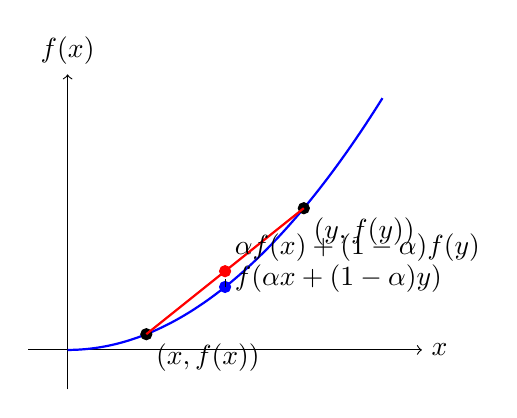
\begin{tikzpicture}
    % Axes
    \draw[->] (-0.5,0) -- (4.5,0) node[right] {$x$};
    \draw[->] (0,-0.5) -- (0,3.5) node[above] {$f(x)$};
    
    % Convex function (parabola)
    \draw[thick, blue] plot [domain=0:4, samples=100] (\x, {0.2*\x*\x});
    
    % Points on the function
    \filldraw[black] (1,0.2) circle (2pt) node[below right] {$(x,f(x))$};
    \filldraw[black] (3,1.8) circle (2pt) node[below right] {$(y,f(y))$};
    
    % Chord
    \draw[red, thick] (1,0.2) -- (3,1.8);
    
    % Midpoint on chord
    \filldraw[red] (2,1) circle (2pt);
    
    % Point on function at same x
    \filldraw[blue] (2,0.8) circle (2pt);
    
    % Vertical line connecting points
    \draw[dashed] (2,0.8) -- (2,1);
    
    % Labels
    \node[right] at (2,0.9) {$f(\alpha x + (1-\alpha)y)$};
    \node[above right] at (2,1) {$\alpha f(x) + (1-\alpha)f(y)$};
  \end{tikzpicture}
  \caption{En konveks funksjon ligger under korden som forbinder to punkter på dens graf}
  \label{fig:convex_function}
\end{figure}

\subsection{Ekvivalente Karakteriseringer}
\begin{theorem}{Karakteriseringer av Konveksitet}{convexity_characterizations}
  For en funksjon $f: C \to \mathbb{R}$ på et konvekst domene $C$:
  \begin{itemize}
    \item \textbf{Førsteordens Betingelse} (når $f$ er deriverbar):
    \[
    f(y)\;\ge\; f(x) + \nabla f(x)^\mathsf{T}\,(y - x), \quad \text{for alle }x, y \in C.
    \]
    Med ord: den lineære approksimasjonen (tangenten) ved $x$ er en global undereestimator av $f$.
    
    \item \textbf{Andreordens Betingelse} (når $f$ er to ganger deriverbar):
    \[
    \nabla^2 f(x)\; \text{er positiv semidefinitt for alle }x \in C.
    \]
    Det vil si at Hessian-matrisen er positiv semidefinitt overalt i $C$.
  \end{itemize}
\end{theorem}

\begin{figure}[htb]
  \centering
  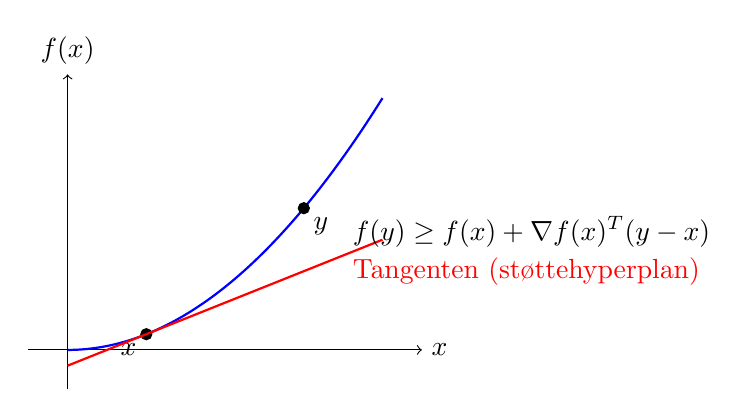
\begin{tikzpicture}
    % Axes
    \draw[->] (-0.5,0) -- (4.5,0) node[right] {$x$};
    \draw[->] (0,-0.5) -- (0,3.5) node[above] {$f(x)$};
    
    % Convex function (parabola)
    \draw[thick, blue] plot [domain=0:4, samples=100] (\x, {0.2*\x*\x});
    
    % Point on the function
    \filldraw[black] (1,0.2) circle (2pt) node[below left] {$x$};
    \filldraw[black] (3,1.8) circle (2pt) node[below right] {$y$};
    
    % Tangent at x
    \draw[red, thick] plot [domain=0:4, samples=100] (\x, {0.2*1*1 + 0.4*1*(\x-1)});
    
    % Labels
    \node[right] at (3.5,1.5) {$f(y) \geq f(x) + \nabla f(x)^T(y-x)$};
    \node[red, right] at (3.5,1) {Tangenten (støttehyperplan)};
  \end{tikzpicture}
  \caption{Førsteordens karakterisering av konveksitet: funksjonen ligger over sine tangentplan}
  \label{fig:first_order}
\end{figure}

\subsection{Eksempler}
\begin{example}{Vanlige Konvekse Funksjoner}{common_convex_functions}
  \begin{itemize}
    \item \textbf{Lineære eller Affine Funksjoner}: $f(x) = c^\mathsf{T} x + \beta$ er konvekse (og også konkave).
    \item \textbf{Normer}: $f(x) = \|x\|_p$ for $p \geq 1$ er konvekse.
    \item \textbf{Kvadratiske Former}: $f(x) = x^\mathsf{T} Q x$ er konveks hvis og bare hvis $Q$ er positiv semidefinitt.
    \item \textbf{Eksponential}: $f(x) = e^{\alpha x}$ (i én dimensjon) eller $f(x)= \exp(\langle \alpha, x \rangle)$ (multidimensjonal) er konveks.
    \item \textbf{Logaritmisk Barriere}: $f(x) = -\log(x)$ på $\mathbb{R}_{++}$ er konveks.
    \item \textbf{Entropi}: $f(x) = x\log(x)$ på $\mathbb{R}_{++}$ er konveks.
  \end{itemize}
\end{example}

\begin{table}[htb]
  \centering
  \begin{tabular}{|l|l|c|}
    \hline
    \textbf{Funksjon} & \textbf{Domene} & \textbf{Konveksitet} \\
    \hline
    $f(x) = c^Tx + b$ & $\mathbb{R}^n$ & Konveks og konkav \\
    $f(x) = \|x\|_p$, $p \geq 1$ & $\mathbb{R}^n$ & Konveks \\
    $f(x) = x^TQx$, $Q \succeq 0$ & $\mathbb{R}^n$ & Konveks \\
    $f(x) = e^x$ & $\mathbb{R}$ & Konveks \\
    $f(x) = -\log(x)$ & $\mathbb{R}_{++}$ & Konveks \\
    $f(x) = x\log(x)$ & $\mathbb{R}_{++}$ & Konveks \\
    $f(x) = 1/x$ & $\mathbb{R}_{++}$ & Konveks \\
    $f(x) = \max\{x_1, x_2, \ldots, x_n\}$ & $\mathbb{R}^n$ & Konveks \\
    \hline
  \end{tabular}
  \caption{Eksempler på vanlige konvekse funksjoner}
  \label{tab:convex_functions}
\end{table}

\subsection{Vanlige Egenskaper}
\begin{theorem}{Operasjoner som Bevarer Funksjonskonveksitet}{function_convexity_preserving}
  Følgende operasjoner bevarer funksjonskonveksitet:
  \begin{itemize}
    \item \textbf{Ikke-negative Vektede Summer}: Hvis $f_1, f_2, \ldots, f_n$ er konvekse og $\alpha_1, \alpha_2, \ldots, \alpha_n \geq 0$, da er $\sum_{i=1}^n \alpha_i f_i$ konveks.
    
    \item \textbf{Punktvis Maksimum}: Hvis $f_1, f_2, \ldots, f_n$ er konvekse, da er $\max\{f_1, f_2, \ldots, f_n\}$ konveks.
    
    \item \textbf{Punktvis Supremum}: Hvis $f_\alpha$ er konveks for hver $\alpha \in A$, da er $\sup_{\alpha \in A} f_\alpha$ konveks.
    
    \item \textbf{Sammensetning med Affin Funksjon}: Hvis $f$ er konveks og $A$ er en matrise og $b$ er en vektor, da er $g(x) = f(Ax + b)$ konveks.
    
    \item \textbf{Minimering over Noen Variabler}: Hvis $f(x,y)$ er felles konveks i $(x,y)$, da er $g(x) = \inf_y f(x,y)$ konveks i $x$.
  \end{itemize}
\end{theorem}

\subsection{Subgradienter (Generelle Derivater)}
\begin{definition}{Subgradient}{subgradient}
  For en konveks funksjon $f: C \to \mathbb{R}$, er en vektor $g \in \mathbb{R}^n$ en \textbf{subgradient} av $f$ ved $x \in C$ hvis
  \[
  f(y)\;\ge\; f(x)\;+\; g^\mathsf{T}\,(y-x),\quad \forall y \in C.
  \]
  Mengden av alle subgradienter av $f$ ved $x$ kalles \textbf{subdifferensialet} av $f$ ved $x$, og betegnes med $\partial f(x)$.
\end{definition}

\begin{figure}[htb]
  \centering
  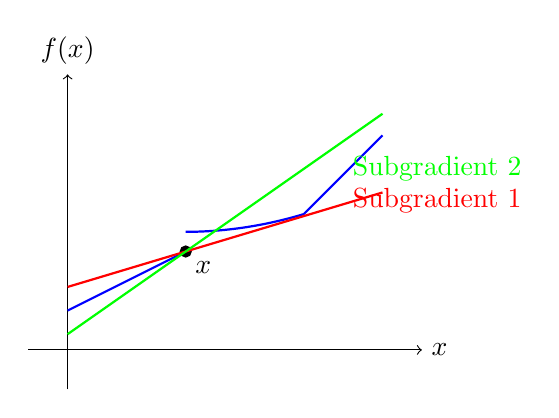
\begin{tikzpicture}
    % Axes
    \draw[->] (-0.5,0) -- (4.5,0) node[right] {$x$};
    \draw[->] (0,-0.5) -- (0,3.5) node[above] {$f(x)$};
    
    % Convex function (piecewise)
    \draw[thick, blue] plot [domain=0:1.5, samples=50] (\x, {0.5*\x + 0.5});
    \draw[thick, blue] plot [domain=1.5:3, samples=50] (\x, {1.5 + 0.1*(\x-1.5)^2});
    \draw[thick, blue] plot [domain=3:4, samples=50] (\x, {1.5 + 0.1*(3-1.5)^2 + 1*(\x-3)});
    
    % Point of non-differentiability
    \filldraw[black] (1.5,1.25) circle (2pt) node[below right] {$x$};
    
    % Subgradients
    \draw[red, thick] plot [domain=0:4, samples=50] (\x, {1.25 + 0.3*(\x-1.5)});
    \draw[green, thick] plot [domain=0:4, samples=50] (\x, {1.25 + 0.7*(\x-1.5)});
    
    % Labels
    \node[red, right] at (3.5,1.9) {Subgradient 1};
    \node[green, right] at (3.5,2.3) {Subgradient 2};
  \end{tikzpicture}
  \caption{Subgradienter av en konveks funksjon ved et punkt der den ikke er deriverbar}
  \label{fig:subgradients}
\end{figure}

\section{Grunnleggende Resultater og Implikasjoner}

\subsection{Jensens Ulikhet}
\begin{theorem}{Jensens Ulikhet}{jensens_inequality}
  For enhver konveks funksjon $f: C \to \mathbb{R}$ og punkter $x_1, x_2, \ldots, x_k \in C$:
  \[
  f\Bigl(\sum_{i=1}^k \alpha_i x_i \Bigr) \;\le\; \sum_{i=1}^k \alpha_i\, f(x_i),
  \]
  når $\alpha_i\ge 0$ og $\sum_{i=1}^k \alpha_i=1$.
  
  For stokastiske variabler, hvis $X$ er en stokastisk variabel med verdier i $C$ og $f$ er konveks, da:
  \[
  f(\mathbb{E}[X]) \leq \mathbb{E}[f(X)]
  \]
  forutsatt at forventningsverdiene eksisterer.
\end{theorem}

\subsection{Konveks Programmering}
\begin{definition}{Konvekst Optimeringsproblem}{convex_optimization_problem}
  Et konvekst optimeringsproblem har formen:
  \begin{mini*}
    {x \in \mathbb{R}^n}{f(x)}{}{}
    \addConstraint{g_i(x) \leq 0,}{i = 1, \ldots, m}
    \addConstraint{h_j(x) = 0,}{j = 1, \ldots, p}
  \end{mini*}
    
  hvor $f$ og $g_i$ er konvekse funksjoner, og $h_j(x) = a_j^Tx - b_j$ er affine funksjoner.
\end{definition}

\begin{theorem}{Egenskaper ved Konveks Optimering}{convex_optimization_properties}
  For et konvekst optimeringsproblem:
  \begin{enumerate}
    \item Enhver lokal minimerer er en global minimerer.
    \item Mengden av minimerere, hvis ikke-tom, er konveks.
    \item Hvis $f$ er strengt konveks, har problemet høyst én løsning.
    \item KKT-betingelsene er nødvendige og tilstrekkelige for optimalitet (under kvalifikasjonsbetingelser).
  \end{enumerate}
\end{theorem}

\subsection{Epigraf-Formulering}
\begin{definition}{Epigraf}{epigraph}
  \textbf{Epigrafen} til en funksjon $f: C \to \mathbb{R}$ er mengden
  \[
  \mathrm{epi}(f) \;=\; \{(x,t)\mid x\in C,\; t\ge f(x)\}.
  \]
  En funksjon $f$ er konveks hvis og bare hvis $\mathrm{epi}(f)$ er en konveks mengde i $\mathbb{R}^{n+1}$.
\end{definition}

\begin{figure}[htb]
  \centering
  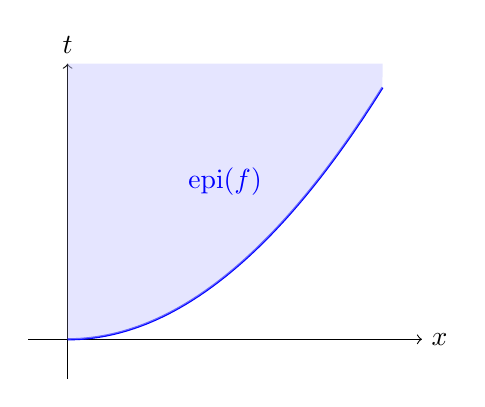
\begin{tikzpicture}
    % Axes
    \draw[->] (-0.5,0) -- (4.5,0) node[right] {$x$};
    \draw[->] (0,-0.5) -- (0,3.5) node[above] {$t$};
    
    % Convex function
    \draw[thick, blue] plot [domain=0:4, samples=100] (\x, {0.2*\x*\x});
    
    % Epigraph
    \fill[blue!20, opacity=0.5] (0,0) -- plot [domain=0:4, samples=100] (\x, {0.2*\x*\x}) -- (4,3.5) -- (0,3.5) -- cycle;
    
    % Label
    \node[blue] at (2,2) {epi$(f)$};
  \end{tikzpicture}
  \caption{Epigrafen til en konveks funksjon}
  \label{fig:epigraph}
\end{figure}

\subsection{Dualitet i Konveks Optimering}
\begin{definition}{Lagrangian-Dualitet}{lagrangian_duality}
  For det konvekse optimeringsproblem
    \begin{mini}
      {x}{f(x)}{}{}
      \addConstraint{g_i(x)}{\leq 0,}{i = 1,\ldots,m}
      \addConstraint{Ax}{= b}{}
    \end{mini}
  er Lagrangian-funksjonen $\mathcal{L}(x,\lambda,\nu) = f(x) + \sum_{i=1}^m \lambda_i g_i(x) + \nu^T(Ax-b)$ hvor $\lambda_i \geq 0$. 
  Dualfunksjonen er $g(\lambda,\nu) = \inf_x L(x,\lambda,\nu)$ og dualproblemet er
    \begin{maxi}
      {\lambda,\nu}{g(\lambda,\nu)}{}{}
      \addConstraint{\lambda}{\geq 0}{}
    \end{maxi}
\end{definition}

\begin{theorem}{Sterk Dualitet}{strong_duality}
  Hvis et konvekst optimeringsproblem tilfredsstiller Slaters betingelse (dvs. det eksisterer et strengt mulig punkt), da gjelder sterk dualitet: de optimale verdiene av primal- og dualproblemet er like.
\end{theorem}

\section{Konveksitet - Sammendrag}
% First table: Basic Concepts
\begin{table}[H]
  \centering
  \begin{tabular}{|p{3cm}|p{5cm}|p{6cm}|}
    \hline
    \rowcolor{blue!25}
    \textbf{Konsept} & \textbf{Definisjon} & \textbf{Matematisk Formulering} \\
    \hline
    Konveks Mengde & En mengde hvor ethvert linjesegment mellom to punkter i mengden ligger helt i mengden &
    \(C\subset \mathbb{R}^n\) er konveks hvis:
    \[\forall x,y\in C,\;\alpha\in [0,1]:\] 
    \[\alpha x + (1-\alpha) y\in C\] \\
    \hline
    \rowcolor{blue!5}
    Konveks Funksjon & En funksjon hvor grafen ligger under linjesegmentet mellom to punkter på grafen &
    \(f: C \to \mathbb{R}\) er konveks hvis:
    \[f(\alpha x + (1-\alpha) y)\;\le\]\[\alpha f(x) + (1-\alpha) f(y)\] 
    for alle \(x,y\in C,\;\alpha\in [0,1]\) \\
    \hline
  \end{tabular}
  \caption{Grunnleggende konsepter innen konveksitet}
  \label{tab:basic_concepts}
\end{table}

% Second table: Characterizations
\begin{table}[H]
  \centering
  \begin{tabular}{|p{3cm}|p{5cm}|p{6cm}|}
    \hline
    \rowcolor{rem-color!25}
    \multicolumn{3}{|l|}{\textbf{Karakteriseringer av Konveksitet}} \\
    \hline
    \rowcolor{rem-color!5}
    1. Ord. Bet. & Tangentapproks. ved ethvert punkt er en global underestimator &
    For deriverbar \(f\), konveksitet er ekvivalent med:
    \[f(y)\;\ge\; f(x) + \nabla f(x)^\mathsf{T} (y - x)\]
    \[\forall x,y \in C\] \\
    \hline
    2. Ord. Bet. & \(H_f(x)\) er pos. semidefinit overalt i \(C\) &
    For \(f \in C^2\), konveksitet er ekvivalent med:
    \[\nabla^2 f(x) \succeq 0\quad \forall x \in C\] \\
    \hline
  \end{tabular}
  \caption{Karakteriseringer av konveksitet}
  \label{tab:characterizations}
\end{table}

% Third table: Important Results
\begin{table}[H]
  \centering
  \begin{tabular}{|p{3cm}|p{5cm}|p{6cm}|}
    \hline
    \rowcolor{cor-color!25}
    \multicolumn{3}{|l|}{\textbf{Viktige Resultater}} \\
    \hline
    \rowcolor{cor-color!5}
    Jensens Ulikhet & Funksjonsverdien av et vektet gjennomsnitt er mindre enn \newline
    eller lik det vektede gjennomsnittet av funksjonsverdiene &
    For konveks \(f\) og vekter \(\alpha_i \geq 0\) med \(\sum_i \alpha_i = 1\):
    \[f\Bigl(\sum_i \alpha_i x_i\Bigr)\;\le\;\sum_i \alpha_i f(x_i)\] \\
    \hline
    Epigraf & Mengden av alle punkter som ligger på eller over grafen til funksjonen &
    \(\mathrm{epi}(f)=\{(x,t) \mid x\in\mathrm{dom}(f), t\ge f(x)\}\)
    
    \(f\) er konveks \(\Leftrightarrow\) \(\mathrm{epi}(f)\) er konveks \\
    \hline
    \rowcolor{cor-color!5}
    Subgradient & Generalisering av gradient for ikke-deriverbare funksjoner &
    En vektor \(g\) er en subgradient av konveks \(f\) ved \(x\) hvis:
    \[f(y)\;\ge\; f(x) + g^\mathsf{T}(y-x)\quad \forall y \in C\] \\
    \hline
  \end{tabular}
  \caption{Viktige resultater innen konveksitet}
  \label{tab:important_results}
\end{table}

% Fourth table: Optimization Theory
\begin{table}[H]
  \centering
  \begin{tabular}{|p{3cm}|p{5cm}|p{6cm}|}
    \hline
    \rowcolor{prop-color!25}
    \multicolumn{3}{|l|}{\textbf{Optimeringsteori}} \\
    \hline
    \rowcolor{prop-color!5}
    Lokale/Globale\newline Minima & For konvekse problemer er\newline ethvert lokalt minimum\newline også et globalt minimum & 
    For konveks \(f\) på konveks \(C\):\newline\quad\(\text{lokal min} \iff \text{global min}\) \\
    \hline
    Sterk Dualitet & Under visse betingelser er det ingen dualitetsgap &
    Under Slaters betingelse: 
    \[\text{primal opt.} = \text{dual opt.}\] \\
    \hline
  \end{tabular}
  \caption{Optimeringsteori og konveksitet}
  \label{tab:optimization_theory}
\end{table}


\section{Betydning i Optimering}
Konveksitet er avgjørende i optimering av flere viktige grunner:

\begin{itemize}
    \item \textbf{Global Optimalitet}: Konvekse optimeringsproblemer har et unikt globalt minimum hvis streng konveksitet holder, siden ethvert lokalt minimum er globalt.
    
    \item \textbf{Forenklede Optimalitetsbetingelser}: Førsteordens optimalitetsbetingelser er tilstrekkelige for global optimalitet, noe som forenkler analyse og løsningsmetoder.
    
    \item \textbf{Algoritmisk Effektivitet}: Det finnes effektive algoritmer for å løse konvekse optimeringsproblemer, inkludert gradientmetoder, indrepunktsmetoder og proksimalmetoder.
    
    \item \textbf{Praktiske Anvendelser}: Mange praktiske problemer innen maskinlæring, kontrollteori, signalbehandling og finans kan formuleres som konvekse optimeringsproblemer eller tilnærmes av dem.
    
    \item \textbf{Dualitetsteori}: Konveksitet muliggjør kraftige dualitetsresultater som gir alternative løsningsmetoder og sensitivitetsanalyse.
\end{itemize}


\paragraph{Oppsummering av Konveksitet}
Konvekse mengder og funksjoner spiller en sentral rolle i optimering fordi de gir problemer som er relativt enkle å analysere og (ofte) mye enklere å løse, både teoretisk og algoritmisk. 
Den viktige egenskapen om at \emph{lokale minima er globale} gjør det mulig å forenkle beregningene betydelig og gir sterke konvergensegenskaper for standardalgoritmer som gradientmetoder, indrepunktsmetoder, subgradientmetoder, og så videre.

\chapter{Hva er optimering?}
\label{chap:what_is_optimization}

Optimering er et felt innen matematikken som handler om å finne den beste løsningen på et gitt problem, enten med eller uten restriksjoner på løsningsrommet.

Målet i et \emph{optimeringsproblem} er å finne en variabel \(x^\star \in \Omega\) som minimerer eller maksimerer en gitt funksjon \(f: \Omega \to \R\),
kalt \emph{mål\-funksjonen} eller \emph{kostnads\-funksjonen}.

\section{Optimeringsproblemer i \texorpdfstring{\(\R^d\)}{Rd}}

Mengden \(\Omega \subseteq \R^d\) betegner de tillatte løsningene og kalles ofte \emph{søkeområdet} eller den \emph{tillatte mengden (eng. feasible set)}.

\begin{definition}{Optimeringsproblemet \((P)\)}{def:optimization_problem}

	La \(f: \Omega \to \R\) være en funksjon vi ønsker å minimere eller maksimere, der \(\Omega \subseteq \R^d\) er mengden av tillatte (mulige) løsninger.
	\[
		\min_{x \in \Omega} f(x) \quad \text{eller} \quad \max_{x \in \Omega} f(x) \tag{P}
	\]

\end{definition}

Vi fokuserer hovedsakelig på minimeringsproblemer, siden maksimeringsproblemer enkelt kan omformuleres ved å erstatte \(f(x)\) med \(-f(x)\).
De fleste algoritmene vi diskuterer, er designet for å løse minimeringsproblemer.

\section{Ubundet og Bundet optimering}
Ulike problemtyper oppstår ut fra hvordan denne mengden \(\Omega\) er definert, og hvilke egenskaper funksjonen \(f\) har.

Vi skiller mellom tre hovedtyper av optimeringsproblemer:
\paragraph{Ubundet optimering} er den enkleste typen optimeringsproblemer, hvor man ikke har restriksjoner på variabelen \(\symbf{x}^\star\), hvor vi ønsker å minimere \(f(x)\) over hele rommet \(\R^d\).
\paragraph{Bundet optimering} er når vi har restriksjoner på den tillatte mengden \(\Omega \subseteq \R^d\). I motsetning til ubundet optimering kan vi ikke lenger søke over hele rommet \(\R^d\), men må holde oss innenfor spesifikke begrensninger.
Disse er ofte definert ved hjelp av ulikheter og likheter.
\begin{align*}
    g_i(x) &\leq 0, \quad i \in \mathcal{I} \quad \text{(ulikhetsrestriksjoner)} \\
    h_j(x) &= 0, \quad j \in \mathcal{E} \quad \text{(likhetsrestriksjoner)}
\end{align*}

Da kan vi definere den tillatte mengden \(\Omega\) som:
\[
    \Omega = \{ x \in \R^d \mid g_i(x) \leq 0, \, i \in \mathcal{I}, \quad h_j(x) = 0, \, j \in \mathcal{E} \}
\]

Under dette igjen kan vi igjen klassifisere 3 bundne optimeringsproblemtyper:
\subparagraph{Lineær programmering (LP)} Når \(f\) og restriksjonene er lineære.
\subparagraph{Ikke-lineær programmering (NLP)} Når én eller flere av \(f\), \(g_i\), eller \(h_j\) er ikke-lineære.
\subparagraph{Kvadratisk programmering (QP)} Når \(f\) er kvadratisk og restriksjonene er lineære.

\paragraph{Konveks optimering} En spesialklasse der \(f\) og \(\Omega\) er konvekse.
Dette forteller oss at enhver lokal løsning er global, løsningen er entydig hvis \(f\) er strengt konveks, og effektive algoritmer finnes.

\section{Globale og lokale løsninger}
\label{sec:global_and_local_solutions}
I optimeringsproblemer er det viktig å skille mellom globale og lokale løsninger. En global løsning er den beste løsningen i hele søkeområdet, mens en lokal løsning er den beste løsningen i et begrenset område rundt et punkt.


\subsection{Globale løsninger}
En global løsning er den beste løsningen i hele søkeområdet \(\Omega\). Dette betyr at det ikke finnes noen annen løsning i hele \(\Omega\) som gir en bedre verdi for funksjonen \(f\).

\begin{definition}{Globale løsninger}{global_solution}

	\medskip
	For en funksjon \(f: \Omega \to \R\) sier vi at \(\symbf{x}^\star \in \Omega\) er en global løsning av minimeringsproblemet~\eqref{eq:global_minimization_problem} hvis:

	\begin{align*}
		f(\symbf{x}^\star) & \leq f(\symbf{x}) \quad \forall \symbf{x} \in \Omega \tag{Global}                                      \\
		f(\symbf{x}^\star) & < f(\symbf{x}) \quad \forall \symbf{x} \in \Omega, \symbf{x} \neq \symbf{x}^\star \tag{Strengt Global}
	\end{align*}
\end{definition}

\subsubsection{Eksistens av globale løsninger}

En funksjon \(f: \Omega \subset \R^d \to \overline{\R}\) har en global løsning (minimum) i \(\Omega\) hvis den er:

\begin{itemize}
	\item \textbf{Nedre semi-kontinuerlig}: For alle \(x \in \Omega\) og alle sekvenser \((x_n)\) som konvergerer mot \(x\):
	      \[
		      f(x) \leq \liminf_{n \to \infty} f(x_n).
	      \]
	\item \textbf{Koersiv}: Det finnes en konstant \(M > 0\) slik at
	      \[
		      f(x) \geq M \quad \forall x \in \Omega.
	      \]
	      Dette sikrer at \(f\) ikke går mot \(-\infty\) når \(x\) går mot uendelig.
\end{itemize}

\begin{theorem}{Eksistens av globale løsninger}{existence_of_global_solution}
	La \(f: \Omega \subset \R^d \to \overline{\R}\) være nedre semi-kontinuerlig og koersiv på \(\Omega\). Da har \(f\) en global løsning (minimum) i \(\Omega\).
\end{theorem}

\subsection{Lokale løsninger}
En lokal løsning er den beste løsningen i et begrenset område rundt et punkt \(\symbf{x}^\star\).
For å avgjøre om \(\symbf{x}^\star\) er en lokal løsning, må vi undersøke om det finnes bedre løsninger i nærheten.
De fleste metoder for dette baseres på Taylor-utvikling \ref{thm:taylors_theorem}.


\begin{definition}{Lokal løsning}{}
	La \(f: \Omega \to \R\) være en funksjon.

	Vi sier at \(x^\star \in \Omega\) er en lokal løsning av optimeringsproblemet hvis, for en viss \(\varepsilon > 0\):

	\begin{align*}
		f(\symbf{x}^\star) & \leq f(\symbf{x}) \quad \forall \; \symbf{x} \in B(\symbf{x}^\star, \varepsilon) \cap \Omega,                                                  \\
		f(\symbf{x}^\star) & < f(\symbf{x}) \quad \forall \; \symbf{x} \in B(\symbf{x}^\star, \varepsilon) \cap \Omega, \symbf{x} \neq \symbf{x}^\star. \tag{Strengt lokal}
	\end{align*}

	hvor \(B(\symbf{x}^\star, \varepsilon)\) er en åpen kule med sentrum \(\symbf{x}^\star\) og radius \(\varepsilon\)~\ref{def:open_ball}.
\end{definition}

\subsubsection{Taylors teorem}
Taylor-utvikling er en metode for å tilnærme en funksjon ved hjelp av dens deriverte.
Den gir oss en måte å uttrykke funksjonen som en sum av dens verdier og deriverte i et punkt, noe som kan være nyttig for å analysere oppførselen til funksjonen i nærheten av det punktet.

Ved hjelp av Taylor-utvikling kan vi avgjøre om \(\symbf{x}^\star\) er en lokal løsning ved å sjekke om gradienten \(\nabla f(\symbf{x}^\star) = 0\) og Hesse-matrisen \(\nabla^2 f(\symbf{x}^\star)\)

\begin{theorem}{Taylors teorem}{taylors_theorem}
	Anta at \(f: \R^n \to \R\) med \(\mathbf{p}\in\R^n\), og la \(t\in[0,1]\).

	\medskip

	Hvis \(f\in\Ccal^1\) (én gang kontinuerlig deriverbar):
	\[
		f(\mathbf{x} + \mathbf{p}) = f(\mathbf{x}) + \nabla f(\mathbf{x}+t\mathbf{p})^\top \mathbf{p},
	\]

	Hvis \(f \in \Ccal^2\) (to ganger kontinuerlig deriverbar):

	\begin{align*}
		\nabla f(\mathbf{x} + \mathbf{p}) = \nabla f(\mathbf{x}) + \int_0^1 \nabla^2 f(\mathbf{x}+t\mathbf{p})\mathbf{p} dt, \\
		\boxed{f(\mathbf{x} + \mathbf{p}) = f(\mathbf{x}) + \nabla f(\mathbf{x})^\top \mathbf{p} + \frac{1}{2}\mathbf{p}^\top \nabla^2 f(\mathbf{x}+t\mathbf{p})\mathbf{p}}
	\end{align*}
\end{theorem}

\subsubsection{Isolerte lokale løsninger}
En isolert lokal løsning er en lokal løsning der det ikke finnes andre løsninger i nærheten. Dette betyr at det er en viss avstand fra \(\symbf{x}^\star\) til alle andre løsninger.

\begin{lemma}{Isolert lokal løsning}{isolated_local_solution}
	La \(f: \Omega \to \R\) være en funksjon.

	Hvis \(\symbf{x}^\star \in \Omega\) er en isolert lokal løsning, finnes det en \(\varepsilon > 0\) slik at:

	\[
		f(\symbf{x}^\star) \leq f(\symbf{x}) \quad \forall \; \symbf{x} \in B(\symbf{x}^\star, \varepsilon) \cap \Omega, \symbf{x} \neq \symbf{x}^\star.
	\]
\end{lemma}


\chapter{Optimalitetsbetingelser}
\label{chap:optimality_conditions}
\section{Første Ordens Nødvendige Betingelser}

For en lokal løsning \(\mathbf{x}^\star\) må gradienten være null:

\begin{theorem}{First-Order Necessary Conditions}{first_order_necessary_conditions}
	Hvis \(\mathbf{x}^\star\) er et lokalt minimum, og \(f\) er kontinuerlig deriverbar rundt \(\mathbf{x}^\star\), da er:
	\[
		\nabla f(\mathbf{x}^\star) = 0.
	\]
\end{theorem}

\section{Andre Ordens Nødvendige Betingelser}

For en lokal løsning må både gradienten være null og Hesse-matrisen positiv definit:

\begin{theorem}{Second-Order Necessary Conditions}{second_order_necessary_conditions}
	Hvis \(\mathbf{x}^\star\) er et lokalt minimum, og \(f\) er to ganger kontinuerlig deriverbar rundt \(\mathbf{x}^\star\), da er:
	\[
		\nabla f(\mathbf{x}^\star) = 0 \quad \text{og} \quad \nabla^2 f(\mathbf{x}^\star) \succeq 0.
	\]
\end{theorem}

\section{Andre Ordens Tilstrekkelige Betingelser}

\begin{theorem}{Second-Order Sufficient Conditions}{second_order_sufficient_conditions}
	Hvis \(\nabla f(\mathbf{x}^\star) = 0\) og \(\nabla^2 f(\mathbf{x}^\star) \succ 0\) (positiv definit), da er \(\mathbf{x}^\star\) et \emph{strengt lokalt minimum}.

	\medskip

	Det vil si at det finnes en \(\varepsilon > 0\) slik at:
	\[
		f(\mathbf{x}^\star) < f(\mathbf{x})  \quad \forall \; \mathbf{x} \in B(\mathbf{x}^\star, \varepsilon) \cap \Omega, \mathbf{x} \neq \mathbf{x}^\star.
	\]
\end{theorem}

\section{Stasjonære punkter}
Stasjonære punkter er punkter der gradienten til funksjonen er null. Dette betyr at det ikke er noen retning der funksjonen øker eller minker, og det kan være et minimum, maksimum eller et sadelpunkt.

\begin{definition}{Stasjonære punkter}{stationary_points}
	La \(f: \Omega \to \R\) være en funksjon. Et punkt \(\symbf{x}^\star \in \Omega\) er et stasjonært punkt hvis:
	\[
		\nabla f(\symbf{x}^\star) = 0.
	\]
	Dette betyr at gradienten til \(f\) i punktet \(\symbf{x}^\star\) er lik null.
\end{definition}

\subsection{Konvergens til stasjonære punkter}
Når vi bruker iterative metoder for å finne minimum av en funksjon \(f\), ønsker vi å vite om algoritmen vil konvergere til det stasjonære punktet \(\symbf{x}^\star\).

\begin{theorem}{Konvergens til stasjonære punkter}{convergence_to_stationary_points}
	Anta at \(f: \R^d \to \R\) er en kontinuerlig deriverbar funksjon, og at følgende betingelser er oppfylt:
	\begin{enumerate}
		\item \(\Omega\) er en lukket og begrenset mengde.
		\item \(f(\symbf{x})\) er koersiv.
		\item \(f(\symbf{x})\) er nedre semi-kontinuerlig.
		\item \(\nabla f(\symbf{x})\) eksisterer og er Lipschitz-kontinuerlig.
		\item \(\nabla^2 f(\symbf{x})\) eksisterer og er Lipschitz-kontinuerlig.
	\end{enumerate}
	Da konvergerer sekvensen \((\symbf{x}_k)\) generert av en optimaliseringsalgoritme til et stasjonært punkt \(\symbf{x}^\star\) i \(\Omega\).
	\[
		\lim_{k \to \infty} \|\nabla f(\symbf{x}_k)\| = 0.
	\]

	hvor \(\symbf{x}_k\) er iteratene generert av en optimaliseringsalgoritme, og \(\symbf{x}^\star\) tilfredsstiller de førsteordens nødvendige betingelsene \(\nabla f(\symbf{x}^\star) = 0\).

\end{theorem}

\section{Optimalitet og konveksitet}
\label{sec:optimality_and_convexity}
For en konveks funksjon \(f\) er det stasjonære punktet \(\mathbf{x}^\star\) også et globalt minimum. Dette er en viktig egenskap ved konvekse funksjoner, og det gjør dem spesielt nyttige i optimering.

\begin{remark}{Konveksitet og stasjonære punkter}{convexity_and_stationary_points}
	\begin{itemize}
		\item Hvis \(f\) er \textbf{konveks} så er alle lokale minimum \(\mathbf{x}^\star\) også globale minimum.
		\item Hvis \(f\) er \textbf{konveks} og \textbf{deriverbar} så er alle stasjonære punkter \(\mathbf{x}^\star\) også globale minimum.
	\end{itemize}
\end{remark}

\begin{example}{Eksistens og optimalitet}{}
	For \( f(x) = x^2 + 2x \), som er kontinuerlig og koersiv, finnes et globalt minimum i \( x^* = -1 \) der \( f(-1) = -1 \).
\end{example}
\begin{example}{Eksistens og optimalitet}{}

	For \( f(x) = x^2 \), har vi \( \nabla f(x) = 2x \). I \( x^* = 0 \) er \( \nabla f(0) = 0 \) og \( \nabla^2 f(x) = 2 > 0 \), som oppfyller SOSC.

\end{example}
